\documentclass[10pt,a4paper]{article}

\usepackage{fontspec}
\usepackage[margin=18mm,headheight=15pt]{geometry}
\usepackage{graphicx}
\usepackage{booktabs}
\usepackage{tabularx}
\usepackage{longtable}
\usepackage{array}
\usepackage{enumitem}
\usepackage{xcolor}
\usepackage{microtype}
\usepackage{fancyhdr}
\usepackage{hyperref}
\usepackage{tikz}
\usepackage{titlesec}
\usepackage{lastpage}
\usepackage{tcolorbox}

\setmainfont{Arial}
\setsansfont{Arial}
\setmonofont{Consolas}

\definecolor{OxfordBlue}{HTML}{315B8A}
\definecolor{CalloutRed}{HTML}{C62828}
\definecolor{OxfordDark}{HTML}{17324D}
\definecolor{OxfordLight}{HTML}{EAF1F8}
\definecolor{OxfordTeal}{HTML}{2D7C82}
\definecolor{OxfordRed}{HTML}{B53932}
\definecolor{SoftGray}{HTML}{F3F5F7}
\definecolor{MidGray}{HTML}{64748B}

\hypersetup{
  colorlinks=true,
  linkcolor=OxfordBlue,
  urlcolor=OxfordTeal,
  pdftitle={Oxford SM4000 Cryostat KULT Public API},
  pdfauthor={Oxford SM4000 Cryostat Library Project}
}

\pagestyle{fancy}
\fancyhf{}
\lhead{\textcolor{OxfordDark}{Oxford SM4000 Cryostat KULT API}}
\rhead{\textcolor{MidGray}{Clarius integration guide}}
\cfoot{\textcolor{MidGray}{\thepage\ / \pageref{LastPage}}}
\renewcommand{\headrulewidth}{0.3pt}

\titleformat{\section}
  {\Large\bfseries\color{OxfordDark}}
  {\thesection}{0.7em}{}
\titleformat{\subsection}
  {\large\bfseries\color{OxfordBlue}}
  {\thesubsection}{0.7em}{}
\titlespacing*{\section}{0pt}{1.7em}{0.7em}
\titlespacing*{\subsection}{0pt}{1.2em}{0.45em}

\setlist[itemize]{leftmargin=1.4em,itemsep=0.25em,topsep=0.3em}
\setlist[enumerate]{leftmargin=1.6em,itemsep=0.35em,topsep=0.35em}
\setlength{\parindent}{0pt}
\setlength{\parskip}{0.45em}
\setlength{\emergencystretch}{2em}
\renewcommand{\arraystretch}{1.18}

\newcommand{\api}[1]{\nolinkurl{#1}}
\newcommand{\statusok}{\textcolor{OxfordTeal}{\textbf{0 = success}}}
\newcommand{\module}[1]{\textcolor{OxfordBlue}{\textbf{\api{#1}}}}

\newtcolorbox{apibox}[1]{
  colback=OxfordLight,
  colframe=OxfordBlue!35,
  coltitle=OxfordDark,
  title=#1,
  fonttitle=\bfseries,
  boxrule=0.5pt,
  arc=1.5mm,
  before upper=\raggedright
}

\newtcolorbox{warningbox}{
  colback=OxfordRed!8,
  colframe=OxfordRed!45,
  coltitle=OxfordRed,
  title=Operational note,
  fonttitle=\bfseries,
  boxrule=0.5pt,
  arc=1.5mm,
  before upper=\raggedright
}

\begin{document}

\begin{titlepage}
  \begin{tikzpicture}[remember picture,overlay]
    \fill[OxfordDark] (current page.north west)
      rectangle ([yshift=-72mm]current page.north east);
    \fill[OxfordBlue] ([yshift=-72mm]current page.north west)
      rectangle ([yshift=-76mm]current page.north east);
  \end{tikzpicture}

  \vspace*{17mm}
  {\color{white}\fontsize{28}{34}\selectfont\bfseries
    Oxford SM4000 Cryostat KULT\par}
  \vspace{2mm}
  {\color{white}\fontsize{20}{25}\selectfont
    Public API and Clarius Cycle Guide\par}

  \vspace{32mm}
  {\Large\bfseries\color{OxfordDark}Purpose}\par
  \vspace{2mm}
  {\large
  Build reproducible Clarius subsites from the public Oxford KULT modules,
  with the Temperature-and-Field cycle as the canonical project pattern.}

  \vspace{14mm}
  \begin{apibox}{Audience}
  4200A-SCS users who consume the compiled
  \api{Oxford_SM4000_Cryo} user library. No knowledge of the Win32 transport,
  ISOBUS framing, or private header implementation is required.
  \end{apibox}

  \vfill
  \begin{tabularx}{\textwidth}{@{}>{\bfseries\color{OxfordDark}}l X@{}}
    Main recipe & Temperature-and-Field subsite cycle \\
    Runtime & Clarius on the Keithley 4200A-SCS \\
    Library & \api{Oxford_SM4000_Cryo} \\
    Document date & 13 November 2026 \\
  \end{tabularx}
\end{titlepage}

\tableofcontents
\newpage

\section{Public API model}

The Oxford library is consumed through Clarius \emph{Custom Actions}. Each
action selects a public module from the \api{Oxford_SM4000_Cryo} user library.
The project tree determines execution order; a cycling Subsite supplies the
current cycle number.

\begin{apibox}{The cycle contract}
The scheduled setters read the current Clarius cycle through
\api{GetKiteCycle()}. Cycle 1 selects array row 1, cycle 2 selects row 2, and
so on. Outside a cycling Subsite, Clarius reports cycle 1, so the same modules
also work normally with a one-element array.
\end{apibox}

The public API exposes measurement values and the selected schedule values.
It does not expose transport stages, Windows error numbers, build markers, or
private device structures. Every module has return type \api{int};
\statusok. A negative return value indicates that the action did not complete.

\subsection{Module summary}

\begin{longtable}{@{}>{\raggedright\arraybackslash}p{0.29\textwidth}
                        >{\raggedright\arraybackslash}p{0.25\textwidth}
                        >{\raggedright\arraybackslash}p{0.40\textwidth}@{}}
\toprule
\textbf{Module} & \textbf{Role} & \textbf{Use in a project} \\
\midrule
\endhead
\module{oxford_initialize} &
Checks the four Oxford devices and applies the IPS field sweep-rate initialization from the reference controller. &
Place once before the cycling Subsite. Do not place it inside the cycle. \\
\addlinespace
\module{oxford_set_temperature} &
Selects a target from the temperature schedule, configures the ITC503, and waits for the reference stability criterion. &
Place near the start of each environment cycle. \\
\addlinespace
\module{oxford_set_magnetic_field} &
Selects a target from the field schedule and performs the reference persistent-magnet procedure. &
Place after temperature and before electrical measurements. \\
\addlinespace
\module{oxford_read_all} &
Returns the combined ILM, ITC, Lambda, and IPS sensor snapshot used by the reference controller. &
Preferred read action when all four Oxford devices are connected. \\
\addlinespace
\module{oxford_read_itc} & Complete ITC503 snapshot. &
Use for focused temperature monitoring or debugging. \\
\addlinespace
\module{oxford_read_ilm} & Complete ILM200 snapshot. &
Use for level monitoring. \\
\addlinespace
\module{oxford_read_lambda} & Lambda controller snapshot. &
Use when Lambda values are required independently. \\
\addlinespace
\module{oxford_read_ips} & Complete IPS120 snapshot. &
Use for detailed magnet and power-supply monitoring. \\
\addlinespace
\module{oxford_set_active} & Sets the ILM probe to the reference active mode. &
Optional project setup action. \\
\addlinespace
\module{oxford_set_standby} & Applies the reference standby sequence and requests zero magnetic field. &
Optional final project action. \\
\bottomrule
\end{longtable}

\section{Canonical Temperature-and-Field project}

The supported main recipe is one saved Clarius project containing one
Temperature-and-Field Subsite. The environment setters, Oxford readback, and
Keithley electrical test are ordered within that Subsite.

\begin{verbatim}
Oxford Temperature and Field Cycle
|-- Initialize
`-- Site
    `-- Temperature and Field Cycle        [Subsite: Cycle]
        |-- Set Temperature
        |-- Set Magnetic Field
        |-- Read All
        `-- Device / Keithley measurement
\end{verbatim}

The Site shown here matches the example project and is useful when the project
also contains devices and electrical tests. The Oxford actions themselves do
not require wafer probing.

\subsection{Create the project}

\begin{enumerate}
  \item Create and load a new blank Clarius project.
  \item From \textbf{Select} $\rightarrow$ \textbf{Actions}, drag a \textbf{Custom Action} to the
        project root. Rename it \textbf{Initialize} and attach
        \api{oxford_initialize}.
  \item From \textbf{Select} $\rightarrow$ \textbf{Wafer Plan}, add a Site and a Subsite. Rename
        the Subsite \textbf{Temperature and Field Cycle}.
  \item Add three Custom Actions beneath the Subsite, in this order:
        \textbf{Set Temperature}, \textbf{Set Magnetic Field}, and
        \textbf{Read All}.
  \item Attach the corresponding public modules from
        \api{Oxford_SM4000_Cryo}.
  \item Add the Keithley device and electrical test after \textbf{Read All}.
  \item Select the Subsite, choose \textbf{Configure}, set
        \textbf{Subsite Operation} to \textbf{Cycle}, and set
        \textbf{Number of Cycles} to the schedule length.
\end{enumerate}

\subsection{Attach an action to the library}

\begin{figure}[htbp]
\centering
\begin{tikzpicture}
  \node[anchor=south west,inner sep=0] (image) at (0,0)
    {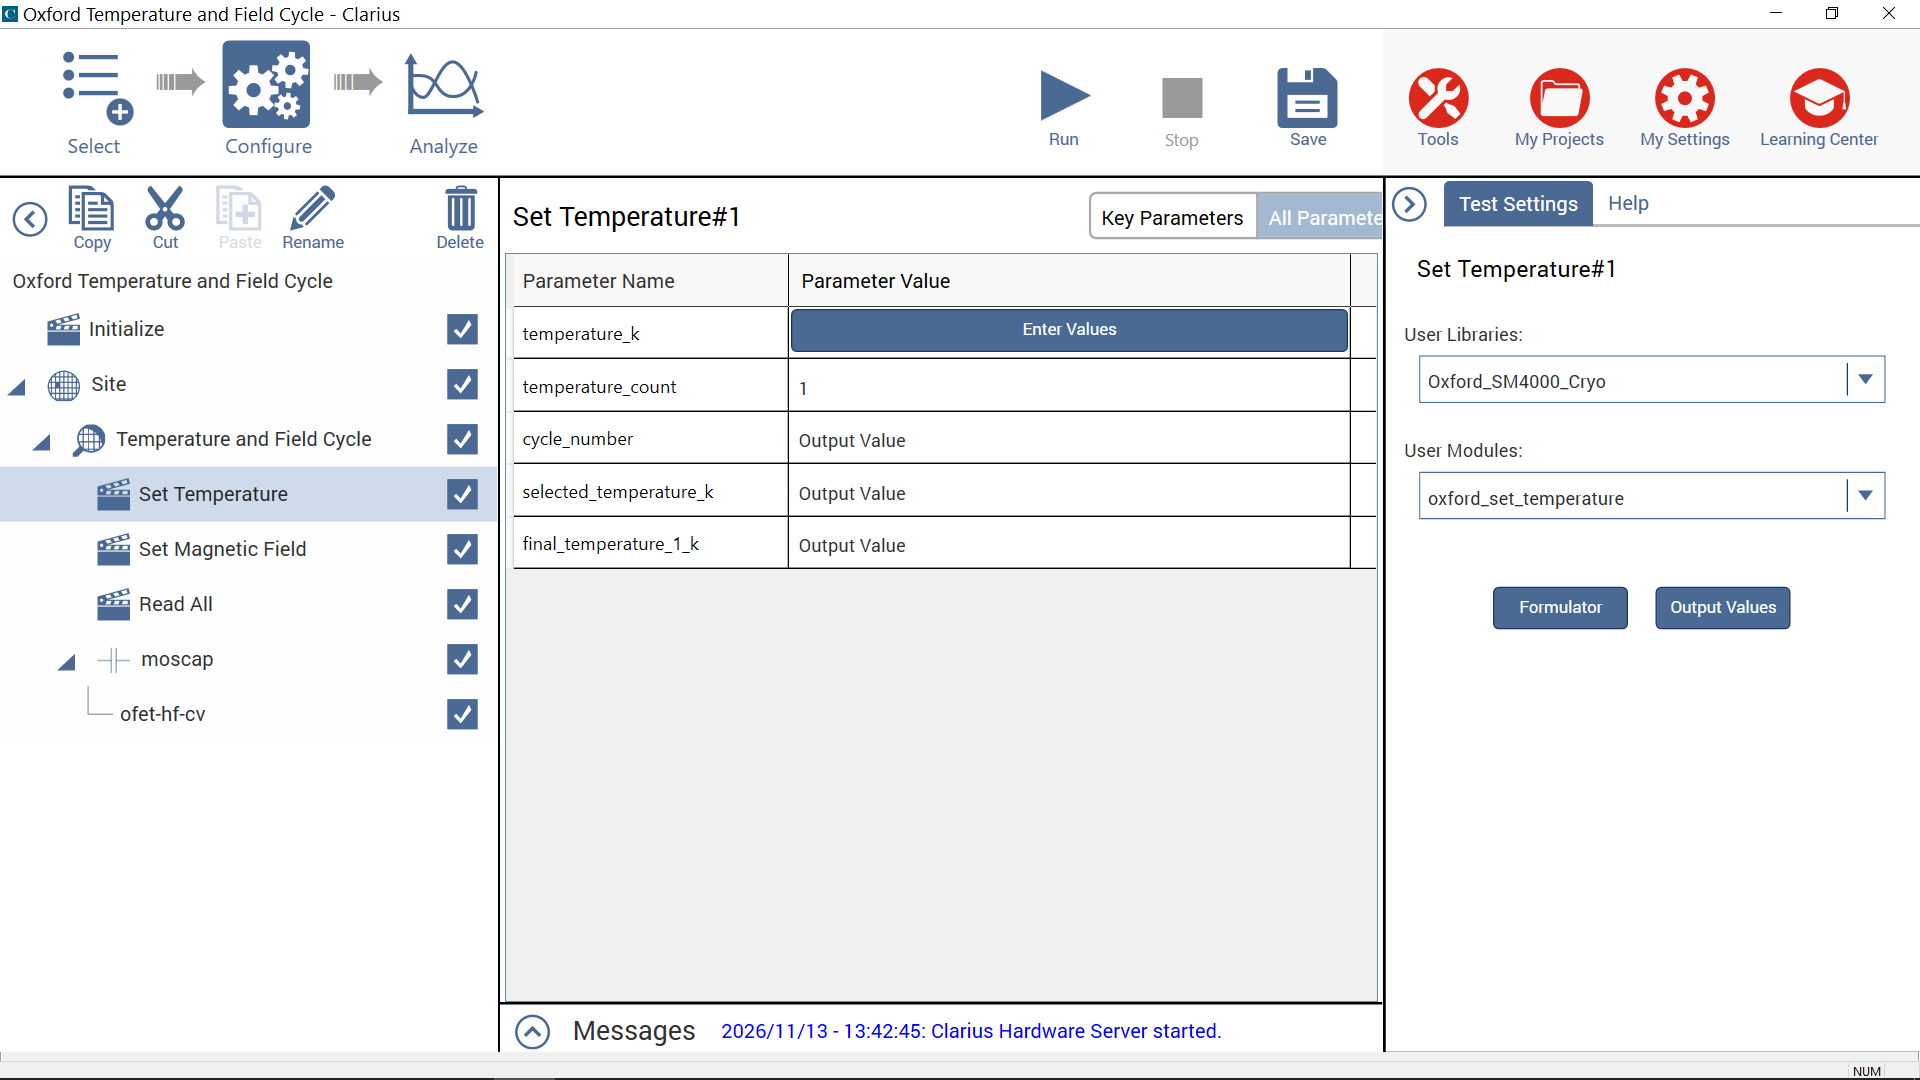
\includegraphics[width=\textwidth]{images/clarius-module-configuration.png}};
  \begin{scope}[x={(image.south east)},y={(image.north west)}]
    \node[circle,fill=CalloutRed,text=white,font=\bfseries,inner sep=2.5pt]
      at (0.235,0.46) {1};
    \node[circle,fill=CalloutRed,text=white,font=\bfseries,inner sep=2.5pt]
      at (0.545,0.31) {2};
    \node[circle,fill=CalloutRed,text=white,font=\bfseries,inner sep=2.5pt]
      at (0.805,0.37) {3};
    \node[circle,fill=CalloutRed,text=white,font=\bfseries,inner sep=2.5pt]
      at (0.865,0.58) {4};
  \end{scope}
\end{tikzpicture}
\caption{Configuring the Set Temperature action. 1: action location in the
project tree; 2: array input in Key Parameters; 3: user library and public
module selection; 4: Output Values selection.}
\label{fig:module-config}
\end{figure}

For every Custom Action, select the action, open \textbf{Configure}, and use
the right-hand \textbf{Test Settings} pane. Select
\api{Oxford_SM4000_Cryo} under \textbf{User Libraries}, then select the module
under \textbf{User Modules}. Figure~\ref{fig:module-config} shows the exact
location of both selectors.

\subsection{Enter paired schedules}

The temperature and field schedules are paired by row. They are not two
independent nested loops. With four Subsite cycles, for example:

\begin{center}
\begin{tabular}{@{}ccc@{}}
\toprule
\textbf{Cycle} & \textbf{\api{temperature_k}} & \textbf{\api{field_t}} \\
\midrule
1 & 4.2 K & 0.0 T \\
2 & 4.2 K & 1.0 T \\
3 & 10.0 K & 0.0 T \\
4 & 10.0 K & 1.0 T \\
\bottomrule
\end{tabular}
\end{center}

Enter the temperature list in \textbf{Set Temperature} and the field list in
\textbf{Set Magnetic Field}. The number of populated rows in both lists must
be at least the configured number of Subsite cycles.

\begin{figure}[htbp]
\centering
\begin{tikzpicture}
  \node[anchor=south west,inner sep=0] (image) at (0,0)
    {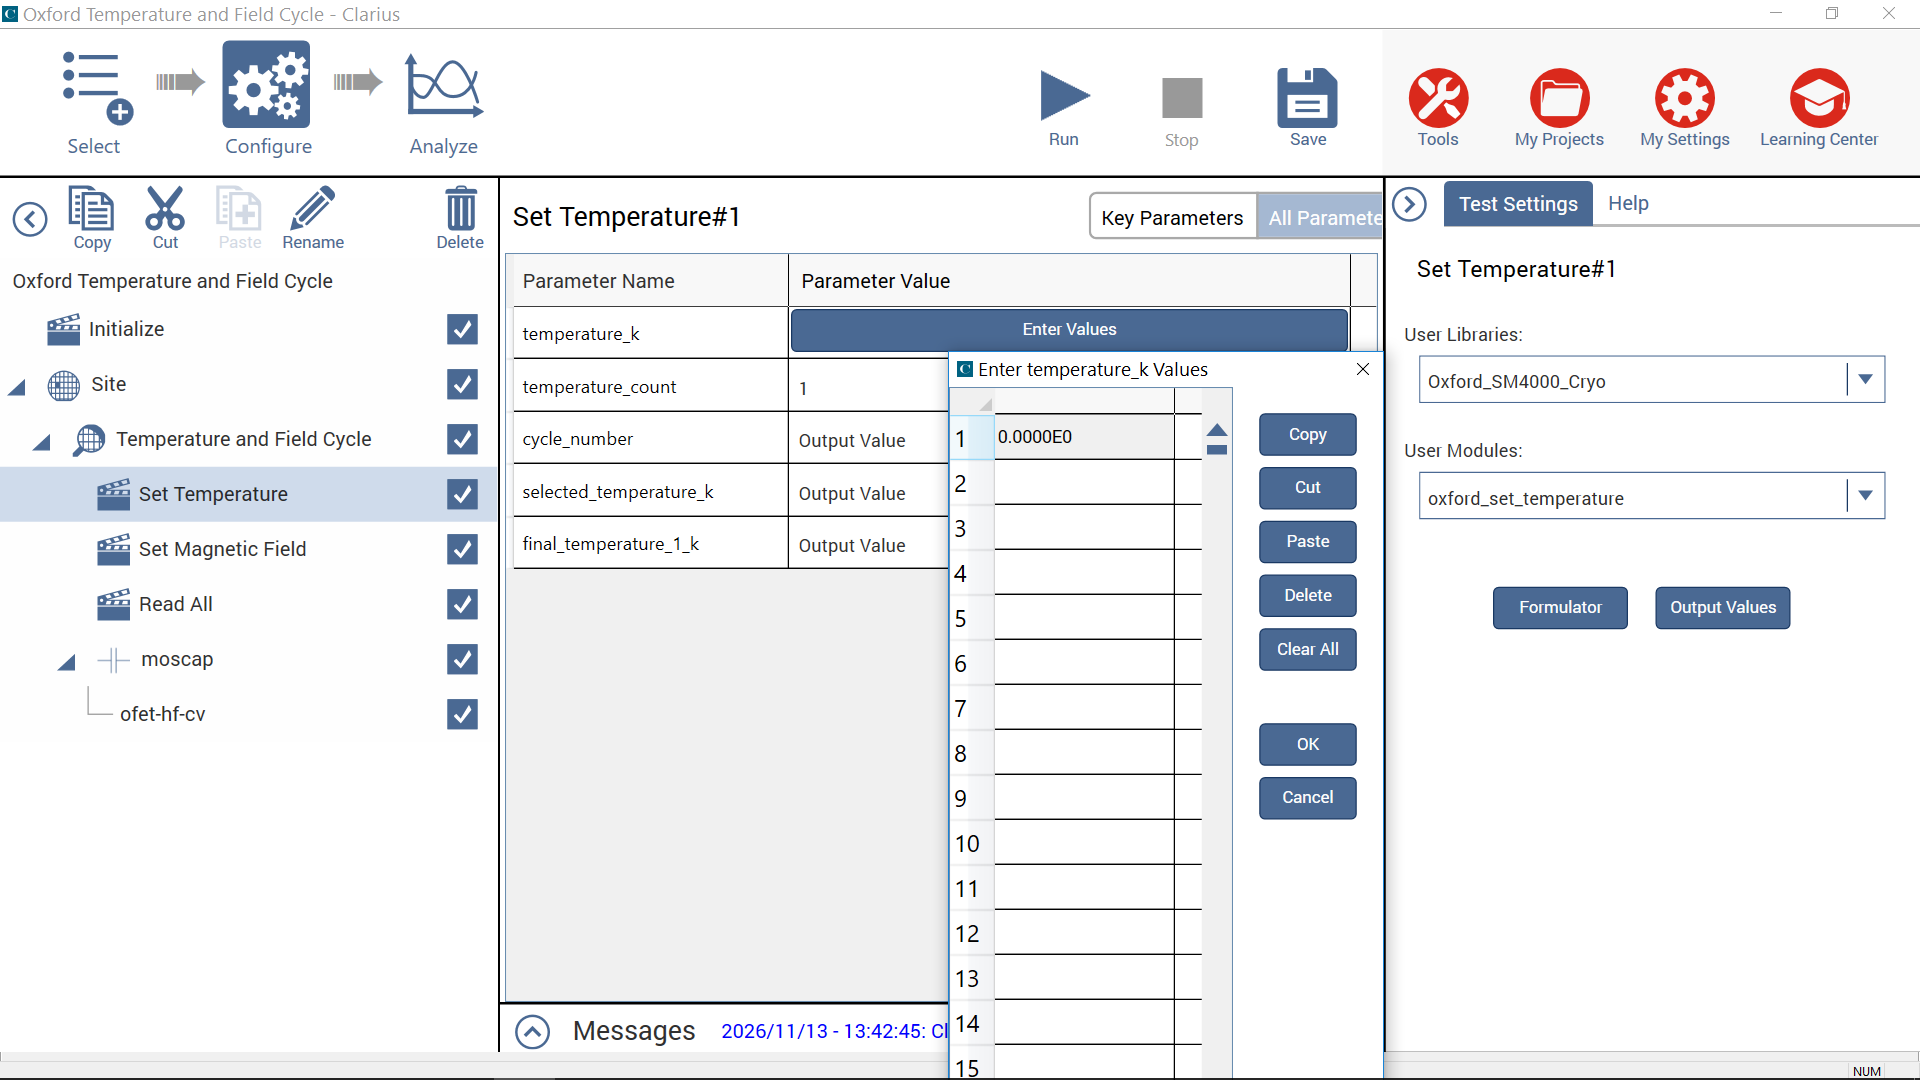
\includegraphics[width=\textwidth]{images/clarius-temperature-array.png}};
  \begin{scope}[x={(image.south east)},y={(image.north west)}]
    \node[circle,fill=CalloutRed,text=white,font=\bfseries,inner sep=2.5pt]
      at (0.555,0.31) {1};
    \node[circle,fill=CalloutRed,text=white,font=\bfseries,inner sep=2.5pt]
      at (0.617,0.48) {2};
    \node[circle,fill=CalloutRed,text=white,font=\bfseries,inner sep=2.5pt]
      at (0.690,0.70) {3};
  \end{scope}
\end{tikzpicture}
\caption{Editing the temperature schedule. 1: Enter Values control;
2: one target per contiguous row; 3: confirm the list with OK. The
\api{temperature_count} value follows the populated input array.}
\label{fig:temperature-array}
\end{figure}

Do not leave blank rows between schedule values. Repeat the same procedure for
\api{field_t}. For a one-point experiment, enter one value in each array and
set the Subsite to one cycle.

\subsection{Execution order}

For each Subsite cycle, Clarius executes the checked children from top to
bottom:

\begin{enumerate}
  \item \api{oxford_set_temperature} selects the current temperature row,
        configures the ITC503, and blocks until the rolling temperature-error
        condition from the reference controller is satisfied.
  \item \api{oxford_set_magnetic_field} selects the corresponding field row
        and completes the persistent-field procedure.
  \item \api{oxford_read_all} records the Oxford environment immediately
        before the electrical measurement.
  \item The Keithley device test runs at the established environment point.
\end{enumerate}

\begin{warningbox}
The magnetic-field action contains the reference 60-second switch-heater
waits and returns the source toward zero after establishing persistent field.
It can therefore take substantially longer than the temperature action or a
normal read action. Do not add it to a monitoring-only cycle.
\end{warningbox}

\section{Public module reference}

\subsection{Initialization and operating mode}

\begin{longtable}{@{}>{\raggedright\arraybackslash}p{0.26\textwidth}
                        >{\raggedright\arraybackslash}p{0.23\textwidth}
                        >{\raggedright\arraybackslash}p{0.43\textwidth}@{}}
\toprule
\textbf{Module} & \textbf{Inputs} & \textbf{Outputs and behaviour} \\
\midrule
\endhead
\module{oxford_initialize} & None &
\api{cycle_number}. Checks ILM200, ITC503, Lambda, and IPS120 communication;
sets the IPS field sweep rate to 0.3382 T/min. \\
\addlinespace
\module{oxford_set_active} & None &
\api{cycle_number}. Sets the ILM probe to FAST using the reference active
sequence. \\
\addlinespace
\module{oxford_set_standby} & None &
\api{cycle_number}, \api{final_source_field_t}. Sets ITC gas and heater
outputs to manual zero, changes the ILM probe to SLOW, and requests zero
magnetic field. \\
\bottomrule
\end{longtable}

\subsection{Scheduled environment setters}

\begin{longtable}{@{}>{\raggedright\arraybackslash}p{0.26\textwidth}
                        >{\raggedright\arraybackslash}p{0.31\textwidth}
                        >{\raggedright\arraybackslash}p{0.35\textwidth}@{}}
\toprule
\textbf{Module} & \textbf{Inputs} & \textbf{Outputs} \\
\midrule
\endhead
\module{oxford_set_temperature} &
\api{temperature_k} (double array), \api{temperature_count} (array size) &
\api{cycle_number}, \api{selected_temperature_k},
\api{final_temperature_1_k} \\
\addlinespace
\module{oxford_set_magnetic_field} &
\api{field_t} (double array), \api{field_count} (array size) &
\api{cycle_number}, \api{selected_field_t},
\api{final_source_field_t} \\
\bottomrule
\end{longtable}

The count parameters are created by KULT as the associated array-size
parameters. The schedule index is \api{cycle_number - 1}. If the current cycle
exceeds the corresponding count, the module returns \api{-21012}.

\subsection{Combined readout}

\module{oxford_read_all} has no inputs. It returns \api{cycle_number} and the
same sensor groups collected by the reference controller:

\begin{longtable}{@{}>{\bfseries\color{OxfordDark}}p{0.18\textwidth}
                        >{\raggedright\arraybackslash}p{0.75\textwidth}@{}}
\toprule
\textbf{Device} & \textbf{Output names} \\
\midrule
\endhead
ILM200 &
\api{helium_percent}, \api{nitrogen_percent} \\
ITC503 &
\api{temperature_1_k}, \api{temperature_2_k}, \api{temperature_3_k},
\api{temperature_setpoint_k}, \api{temperature_error_k},
\api{gas_percent}, \api{heater_volts} \\
Lambda &
\api{lambda_pressure_mbar}, \api{lambda_temperature_k},
\api{lambda_valve_percent} \\
IPS120 &
\api{current_output_a}, \api{current_setpoint_a},
\api{magnet_current_a}, \api{persistent_current_a}, \api{trip_current_a},
\api{field_output_t}, \api{field_setpoint_t}, \api{persistent_field_t},
\api{trip_field_t}, \api{supply_voltage_v},
\api{switch_heater_current_ma} \\
\bottomrule
\end{longtable}

Use the action's \textbf{Output Values} button to select only the columns that
should be promoted into the Subsite Analyze sheet.

\subsection{Individual read modules}

The individual readers have no inputs and always return \api{cycle_number}.
They are useful for focused projects and for installations where not all four
Oxford devices are connected.

\begin{longtable}{@{}>{\raggedright\arraybackslash}p{0.24\textwidth}
                        >{\raggedright\arraybackslash}p{0.69\textwidth}@{}}
\toprule
\textbf{Module} & \textbf{Output groups} \\
\midrule
\endhead
\module{oxford_read_ilm} &
Channel usage/status, relay status, helium and nitrogen levels, channel
currents, and valve position. \\
\addlinespace
\module{oxford_read_itc} &
ITC state, temperatures 1--3, setpoint, error, heater percentage/voltage,
gas percentage, and P/I/D settings. \\
\addlinespace
\module{oxford_read_lambda} &
Lambda state, pressure, temperature, and valve position. \\
\addlinespace
\module{oxford_read_ips} &
IPS state; current, field, sweep, persistent, trip, voltage, switch-heater,
lead-resistance, and magnet-inductance values. \\
\bottomrule
\end{longtable}

\section{Demo patterns}

These are demonstrations of the same public API, not additional required
projects.

\subsection{One-point operation without cycling}

Place \api{oxford_set_temperature}, \api{oxford_set_magnetic_field}, and
\api{oxford_read_all} directly in a project. Enter one temperature and one
field value. With no active Subsite cycle, \api{GetKiteCycle()} returns 1, so
the first array row is used.

\subsection{Read-only monitoring cycle}

Create a cycling Subsite containing only \api{oxford_read_all} and any desired
Keithley measurement. Set the number of cycles and cycle delay in the Subsite
configuration. This records the environment without changing temperature or
field.

\subsection{Focused device demo}

For initial commissioning, use \api{oxford_read_itc} and
\api{oxford_read_ilm} independently. This avoids making a combined read depend
on Lambda and IPS availability.

\section{Building a custom cycle safely}

Users may rearrange the public modules, but should preserve the following
rules:

\begin{enumerate}
  \item Put \api{oxford_initialize} outside the cycling Subsite.
  \item Keep environment-changing actions before electrical measurements.
  \item Keep temperature and field schedules contiguous and at least as long
        as the Subsite cycle count.
  \item Treat schedule rows as paired environment points.
  \item Use \api{oxford_read_all} immediately before the electrical test when
        a synchronized environment record is required.
  \item Use individual readers when only part of the Oxford system is
        connected.
  \item Preserve project recipes by copying the Clarius project before
        changing schedules. The compiled KULT library is shared; action
        parameter values belong to the project instance.
\end{enumerate}

\section{Return status and common configuration errors}

The module return value is the public status interface. There are no separate
build, transport-stage, or Windows-error output parameters.

\begin{tabularx}{\textwidth}{@{}>{\bfseries\color{OxfordDark}}l X@{}}
\toprule
\textbf{Status} & \textbf{Meaning and response} \\
\midrule
0 & Action completed successfully. \\
-21009 & An Oxford device returned a response beginning with ``?''. Check the
command applicability and device operating state. \\
-21012 & The active cycle number exceeds the schedule length. Increase the
array length or reduce the Subsite cycle count. \\
Other negative value & Communication, response, configuration, or close
failure. Confirm COM1, cable power through DTR/RTS, and the connected device. \\
\bottomrule
\end{tabularx}

\begin{apibox}{Recommended commissioning sequence}
First run \api{oxford_initialize}; then run \api{oxford_read_itc} and
\api{oxford_read_ilm}; then test one temperature-field point; finally enable
the complete schedule and electrical measurement.
\end{apibox}

\end{document}
